\section{Constraints}\label{section:constraints}
The purpose of this section is to describe a set of constraints. 
The reason for doing so, is the limited time allotted for the project. 
The constraints that are applied to the project have each been depicted in \figref{figure:constraints}.
Each constraint is explained below, the letter in the list corresponds to the letter in \figref{figure:constraints}.  

\begin{enumerate}[label=(\alph*),itemsep=2pt,parsep=2pt]
%\item Jitter noise is caused by tiny vibrations and occurs when the player is handling the device.
%Therefore, the application will ignore all gravitational-values between -0.1 g and 0.1 g.
\item To simplify the complexity of the application, the movement-area for the player will be a fixed size of $300 cm$ in width.
It means that the player will have to play within the movement-area.
%\item To help the application decide whether a step is actually a step, the maximum length of a step is limited to 100 cm.
%\item The minimum length of a step is set to 20 cm.
\item To ensure consistency in accelerometer readings, a player must hold the device in landscape mode, with the touch pad buttons to the right and the x-axis in a vertical line. As it is impossible to keep the phone completely steady while moving, the application will allow for a rotation of up to $30^\circ$ around the x- and z-axis.
\item The maximum velocity is limited to $3 m/s$, as the player should not be able to move faster than this.
\item Acceleration is constrained to $1 g$. From observations, accelerations with a value exceeding $1 g$ does not happen while side stepping, this includes both negative and positive acceleration values.
\end{enumerate}

\begin{figure}[h]
	\centering
	%---- linebreak	
	\begin{subfigure}[b]{0.45\textwidth}
		\centering
		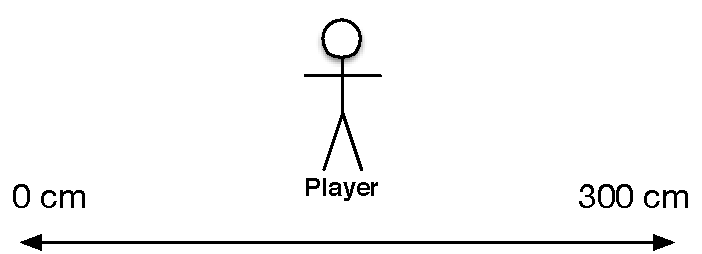
\includegraphics[scale = 0.45]{media/constraints/02-fixed-movement-area}
		\caption{Fixed movement area.}
		\label{figure:fixed-movement-area}
	\end{subfigure}
	\qquad
	\begin{subfigure}[b]{0.45\textwidth}
		\centering
		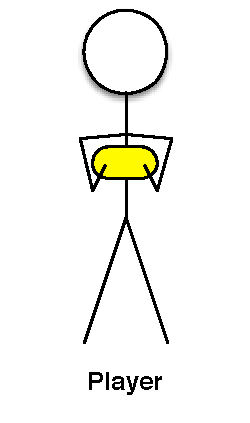
\includegraphics[scale = 0.45]{media/constraints/05-fixed-device-position}
		\caption{Fixed device position.}
		\label{figure:fixed-device-position}
	\end{subfigure}
	%---- linebreak
	\begin{subfigure}[b]{0.45\textwidth}
		\centering
		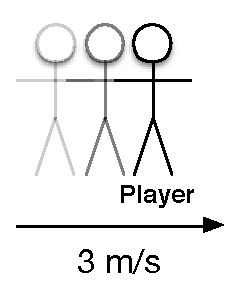
\includegraphics[scale = 0.45]{media/constraints/06-maximum-velocity}
		\caption{Maximum velocity.}
		\label{figure:maximum-velocity}
	\end{subfigure}
	\qquad
	\begin{subfigure}[b]{0.45\textwidth}
		\centering
		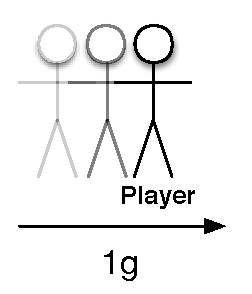
\includegraphics[scale = 0.45]{media/constraints/07-maximum-acceleration}
		\caption{Maximum acceleration.}
		\label{figure:maximum-gravitational-pull}
	\end{subfigure}		
	\caption{Constraints}
	\label{figure:constraints}
\end{figure}